\section{Model Augmentation with GPR Models}\label{aug}
In this section, we demonstrated the application of GPR on stellar model augmentation.  

\subsection{Training GPR Models}

To demonstrate our work flow, we present the training process of a GPR model for the effective temperature with 2-demission inputs ($M$, $t_{\rm frac}$). The grid used here includes stellar models with fixed $[Fe/H]_{\rm init}$ (0.0 dex), $Y_{\rm init}$ (0.28), and $\alpha_{\rm MLT}$ (2.1). The total number of models is 24,485.  

\subsubsection{Step1: Selecting Training, Testing, and Validating Data}

For properly training and validating a GPR model, three types of data are required. Firstly, training data are used to train a GPR model. Because the computational and memory complexity exponentially increase with the number of training data, a practical limit is about 10,000. Secondly, we required a testing data set, which were also selected from the model grid but not used in any training processes. Testing data are used to examine wether a GPR model gives proper description for the model grid. Once a GPR model provides good agreement with the testing data, the training succeeds. The last is validating data, which were randomly distributed in the input parameters space. Validating data are used to validate the GPR model performance and estimate the systematical uncertainty.

We selected these three model data following one principle: the data uniformly distribute on all evolutionary stages. Due to the step-control strategy, our \textsc{MESA} models do not uniformly distribute. Models are dense at the main-sequence and the red-giant phases but quite sparse on subgiant stage. Random sampling is hence not appropriate. 
We tested a few methods and lastly used the gradient on the $T_{\rm eff}$ - $\log g$ diagram as the weights for sampling.  For each evolutionary track, we calculated the gradient as $\delta d$ = $(\delta T_{\rm eff}^{2}$ + $\delta \log g^{2})^{1/2}$, which gives relatively uniform data distribution. Selected data for training the 2-demission inputs GPR model are  demonstrated in Figure~\ref{fig:data_on_hrd} . We selected 3,000 on-grid models as training data, reserved 5,000 on-grid models as testing data, and sampled 5,000 off-grid models as validating data.

\begin{figure}
	\includegraphics[width=1.0\columnwidth]{2D_data_on_HR.pdf}
    \caption{Selected training and testing data for the GPR model with 2-demission inputs on the $T_{\rm eff}$ - $\log g$ (Top) and $M$ - $t_{\rm frac}$ (bottom) diagrams. Black and red dots represent training and testing data. }
    \label{fig:data_on_hrd}
\end{figure}

\subsubsection{Step 2: Training the Primary GPR Model with the MLP Kernel}

We trained a GPR model with the MLP kernel. The GPR model function is demonstrated in Figure~\ref{fig:gpmodel}. 

We used testing data to examine wether the model gives proper description for the grid.  
The $T_{\rm eff} $ residuals of 95\% models are below 1K. This indicate that the MLP kernel is appropriate for the data. However, the GPR model does not well reproduce the features for $M$ > 1.1 and $t'$ = 5 -- 6.  This corresponds to the 'hook' and the turn-off point on the  $T_{\rm eff} - \log g$ diagram shown at the bottom. 

\begin{figure}
	% To include a figure from a file named example.*
	% Allowable file formats are eps or ps if compiling using latex
	% or pdf, png, jpg if compiling using pdflatex
	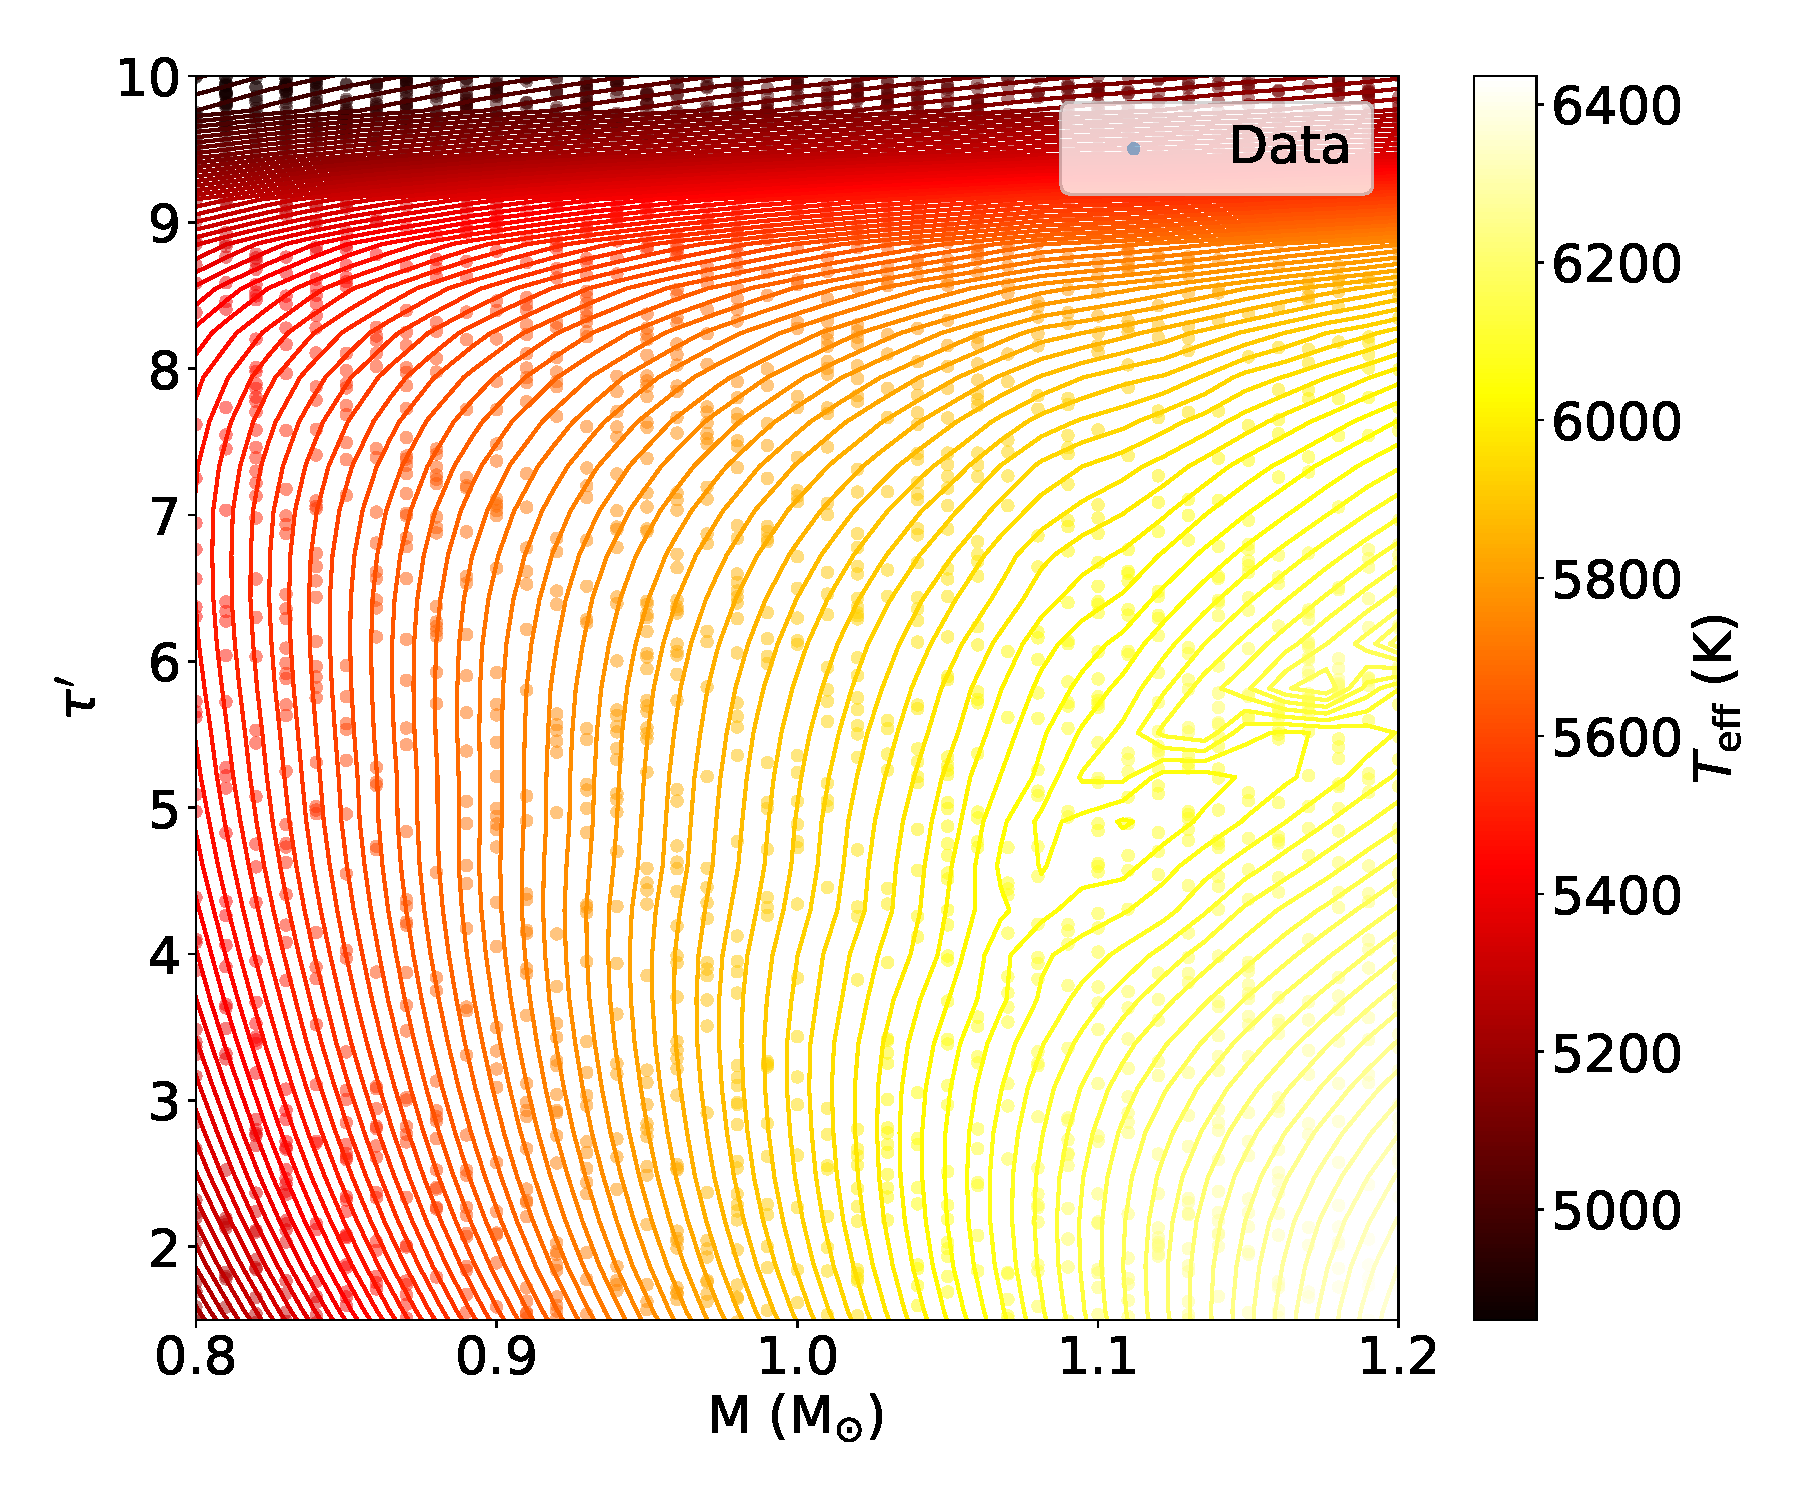
\includegraphics[width=1.0\columnwidth]{2d_gpmodel_MLP.pdf}
    \caption{Top: The GPR model (using the MLP kernel) for the effective temperature ($T_{\rm eff}$) as a function of mass ($M$) and age index ($t'$). Grey counters describes the original grid and coloured counters are GPR predictions. Note that grey counters are interpolated based on the model grid, hence they are not very smooth. Bottom: Residuals of the GPR model on the $T_{\rm eff} - \log g$ diagram.}  
    \label{fig:gpmodel}
\end{figure}

\begin{figure}
	% To include a figure from a file named example.*
	% Allowable file formats are eps or ps if compiling using latex
	% or pdf, png, jpg if compiling using pdflatex
	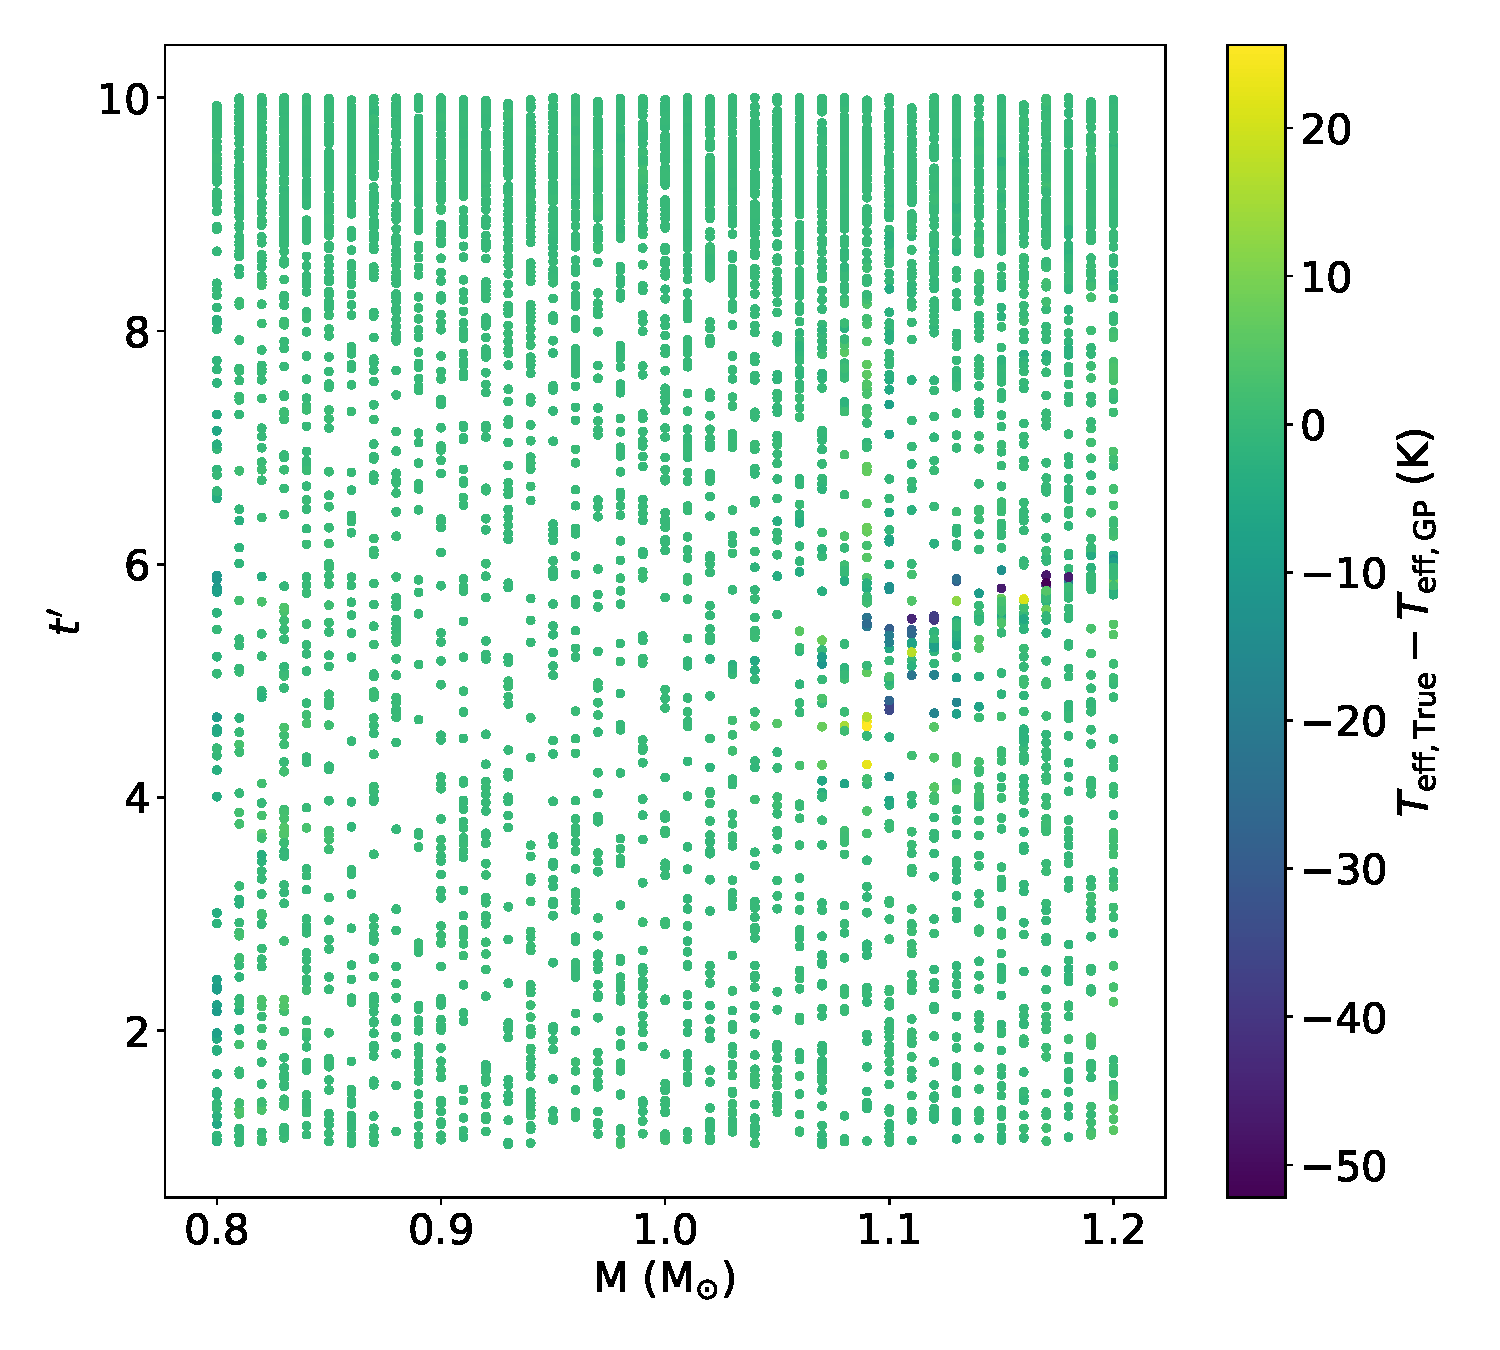
\includegraphics[width=1.0\columnwidth]{M0_ongrid_validation.pdf}
    \caption{Validation (on-grid) for the GPR model.}  
    \label{fig:validation0l}
\end{figure}



\subsubsection{Step3: Training GPR Models for Residuals}

We then worked on an additional GPR model to fit residuals. 

As it can be seen in Figure~\ref{fig:residuals}., the residuals are mostly close to zero in the parameter space and only arise in some particular areas. They hence can be treated as 'spikes'. We selected a number of kernels which are suitable for spike data (MLP, EXP, RQ, Mat32, and RBF), used each them to fit the residuals, and examined which one gives best predictions. The validation (on-grid) errors of each GPR model are illustrated in Figure~\ref{fig:residual}. As it shown that the combined GPR model with the MLP kernel for data and the RBF kernel for residuals gives the best predictions. 

\begin{figure}
	% To include a figure from a file named example.*
	% Allowable file formats are eps or ps if compiling using latex
	% or pdf, png, jpg if compiling using pdflatex
	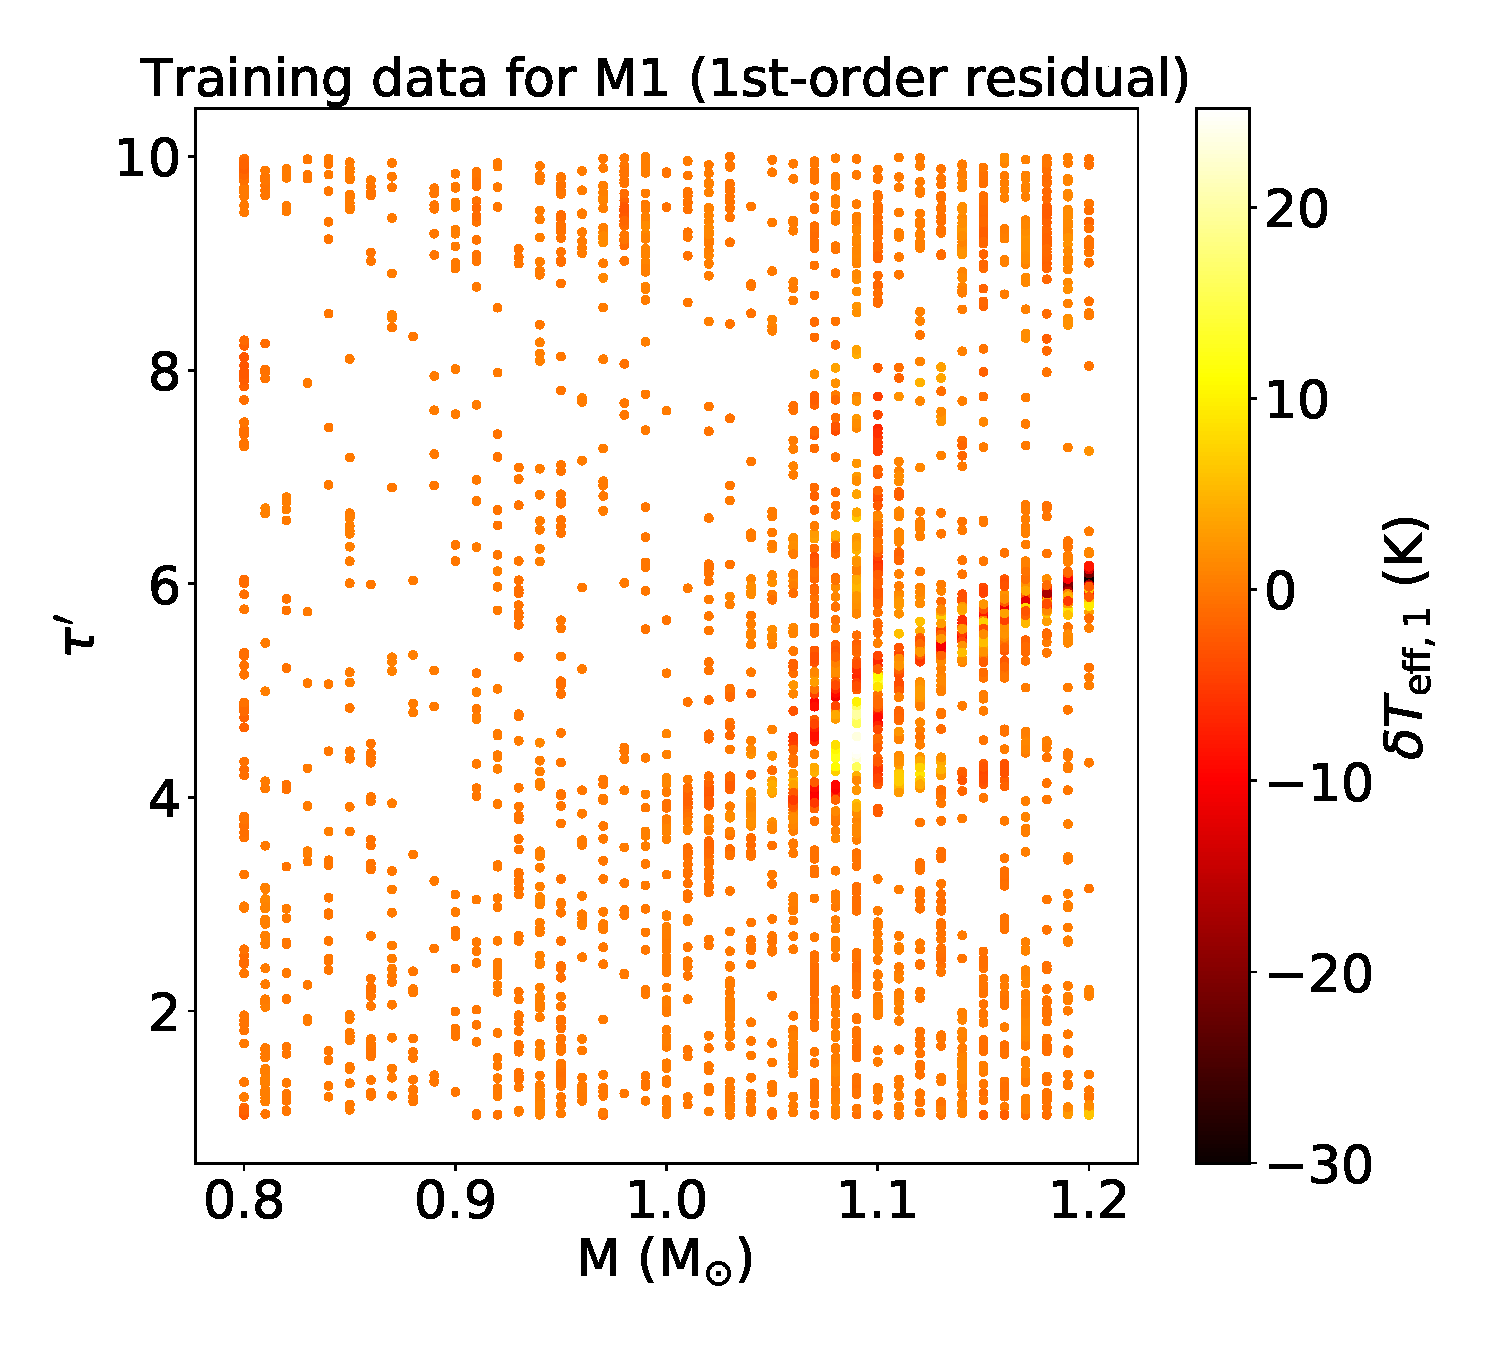
\includegraphics[width=1.0\columnwidth]{M1_data.pdf}
	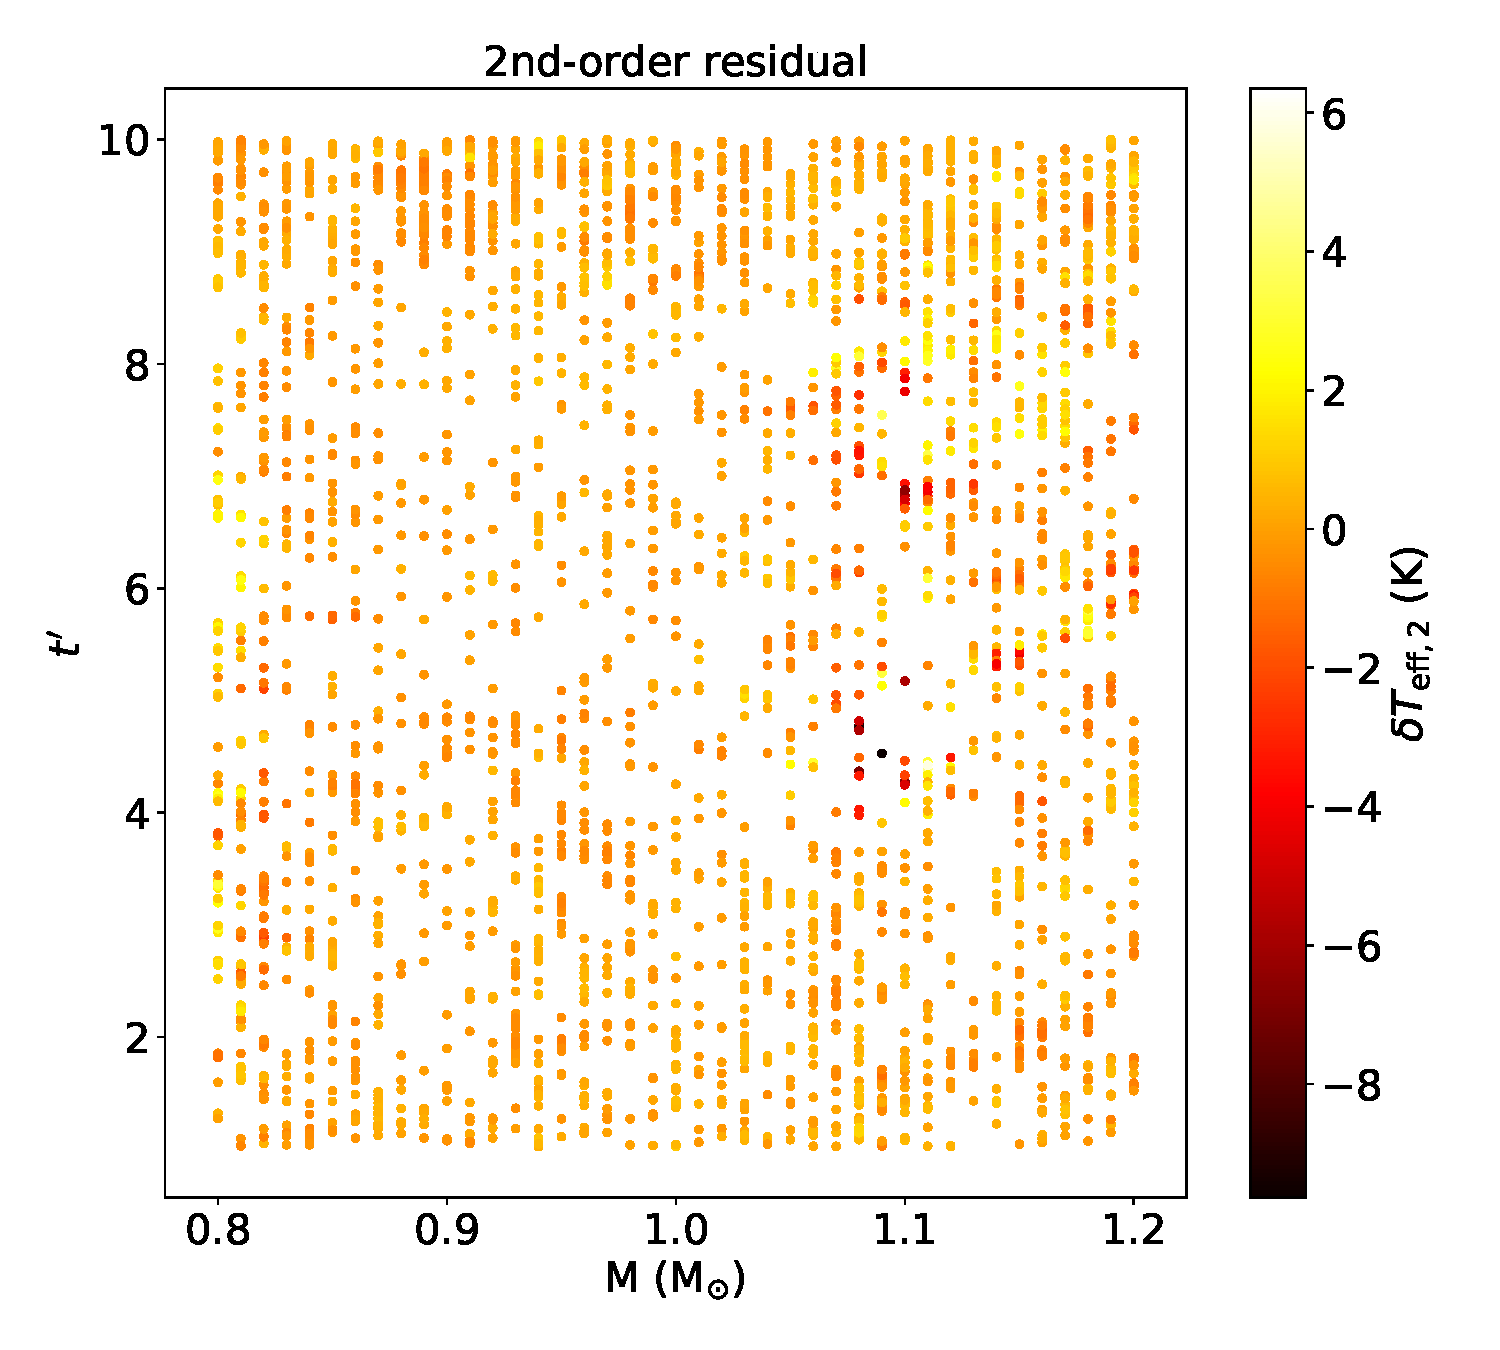
\includegraphics[width=1.0\columnwidth]{M2_data.pdf}
    \caption{Training data for the first and second order residuals.}  
    \label{fig:residualsl}
\end{figure}

 \begin{figure}
	% To include a figure from a file named example.*
	% Allowable file formats are eps or ps if compiling using latex
	% or pdf, png, jpg if compiling using pdflatex
	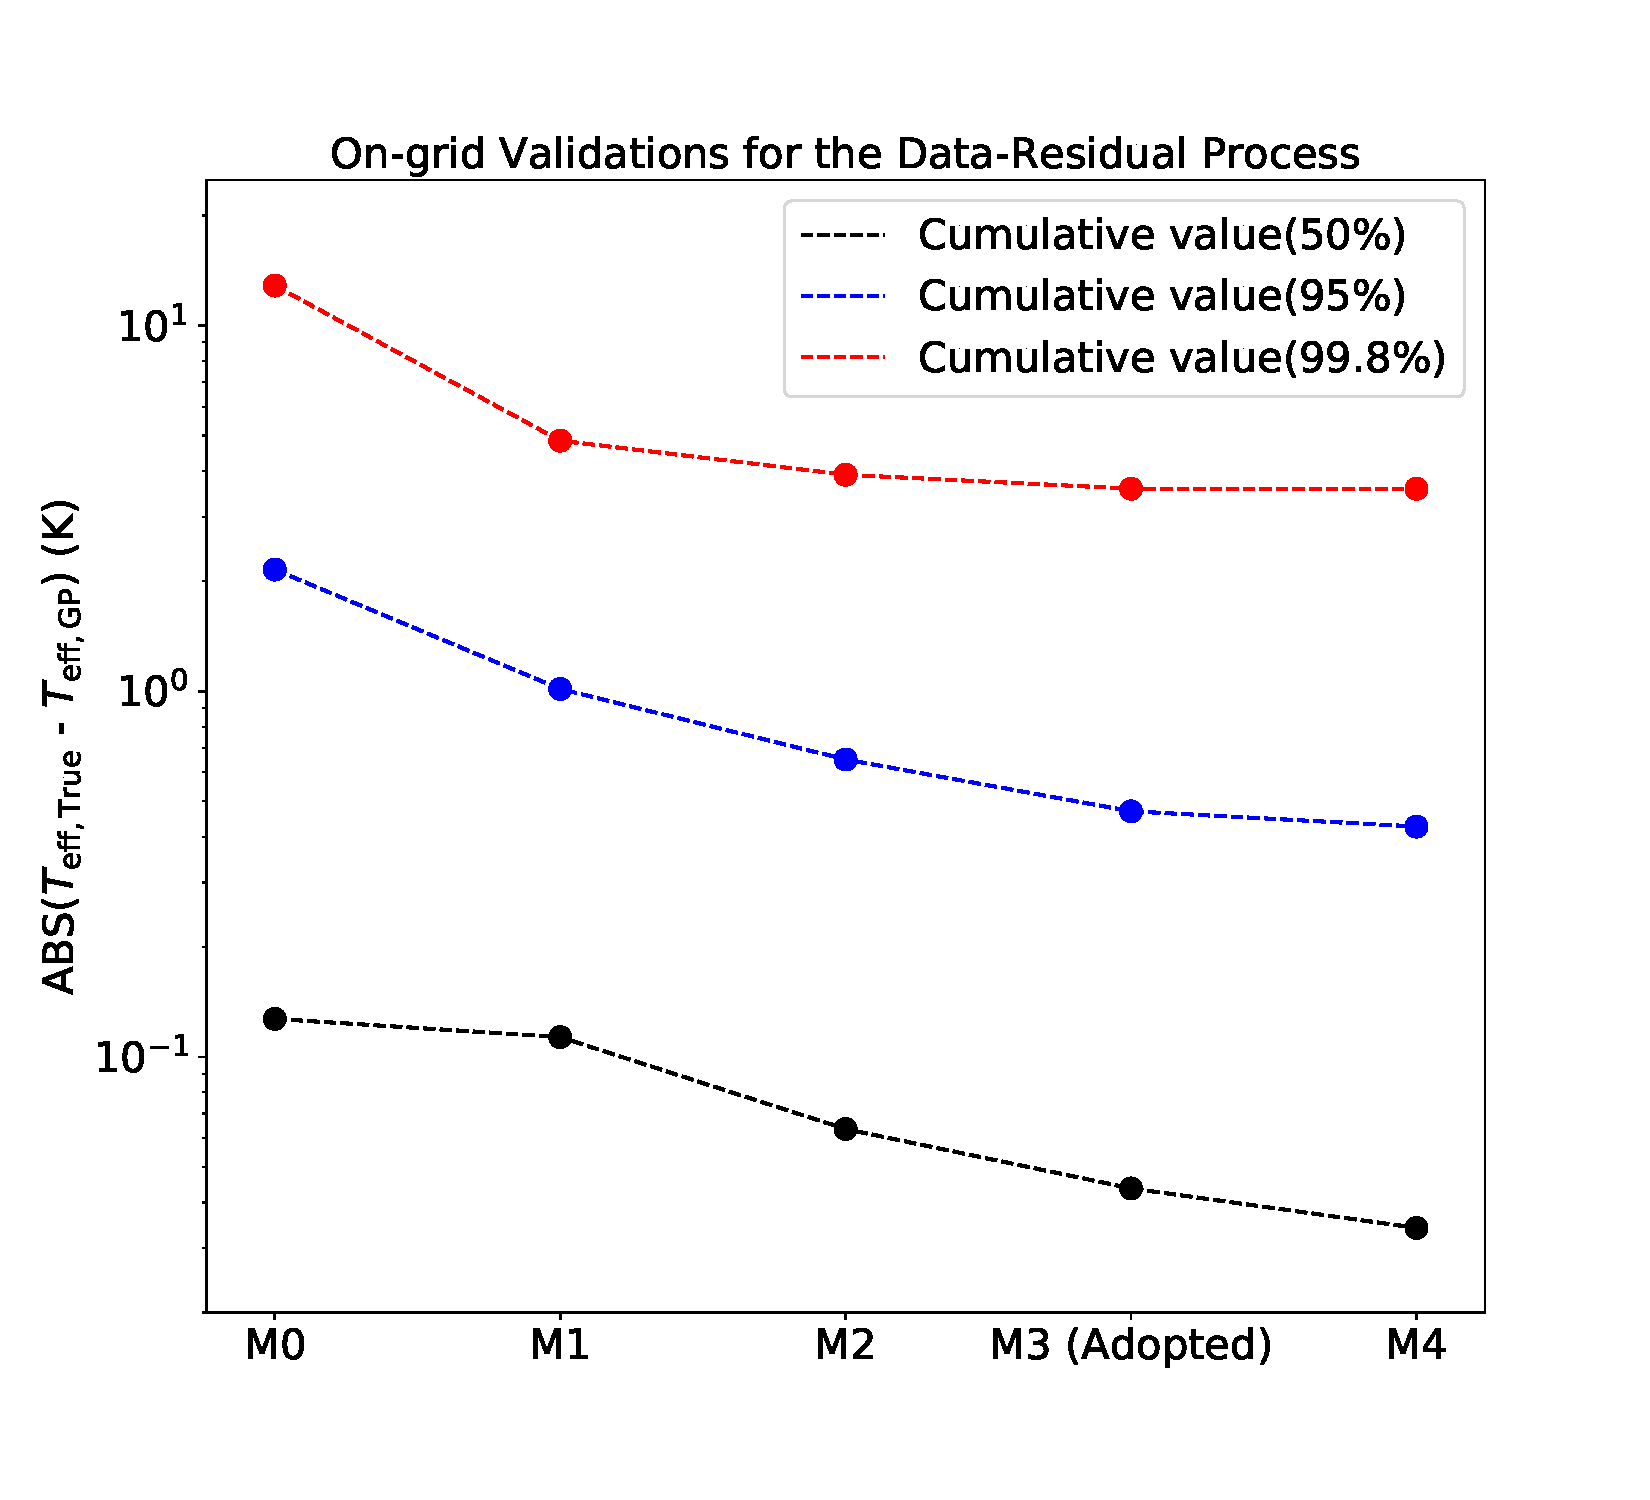
\includegraphics[width=1.0\columnwidth]{all_validations.pdf}
    \caption{On-grid validations.}  
    \label{fig:on-grid_validation}
\end{figure}

\subsubsection{Validating the GPR Model and Estimating Systematical Uncertainty}

We lastly validated the GPR model obtained in the previous step (kernel is MLP/RBF) with off-grid stellar models. The distribution of offsets between true values and the GPR predictions are shown in Figure~\ref{fig:2d_validation}. 
 
 \begin{figure}
	% To include a figure from a file named example.*
	% Allowable file formats are eps or ps if compiling using latex
	% or pdf, png, jpg if compiling using pdflatex
	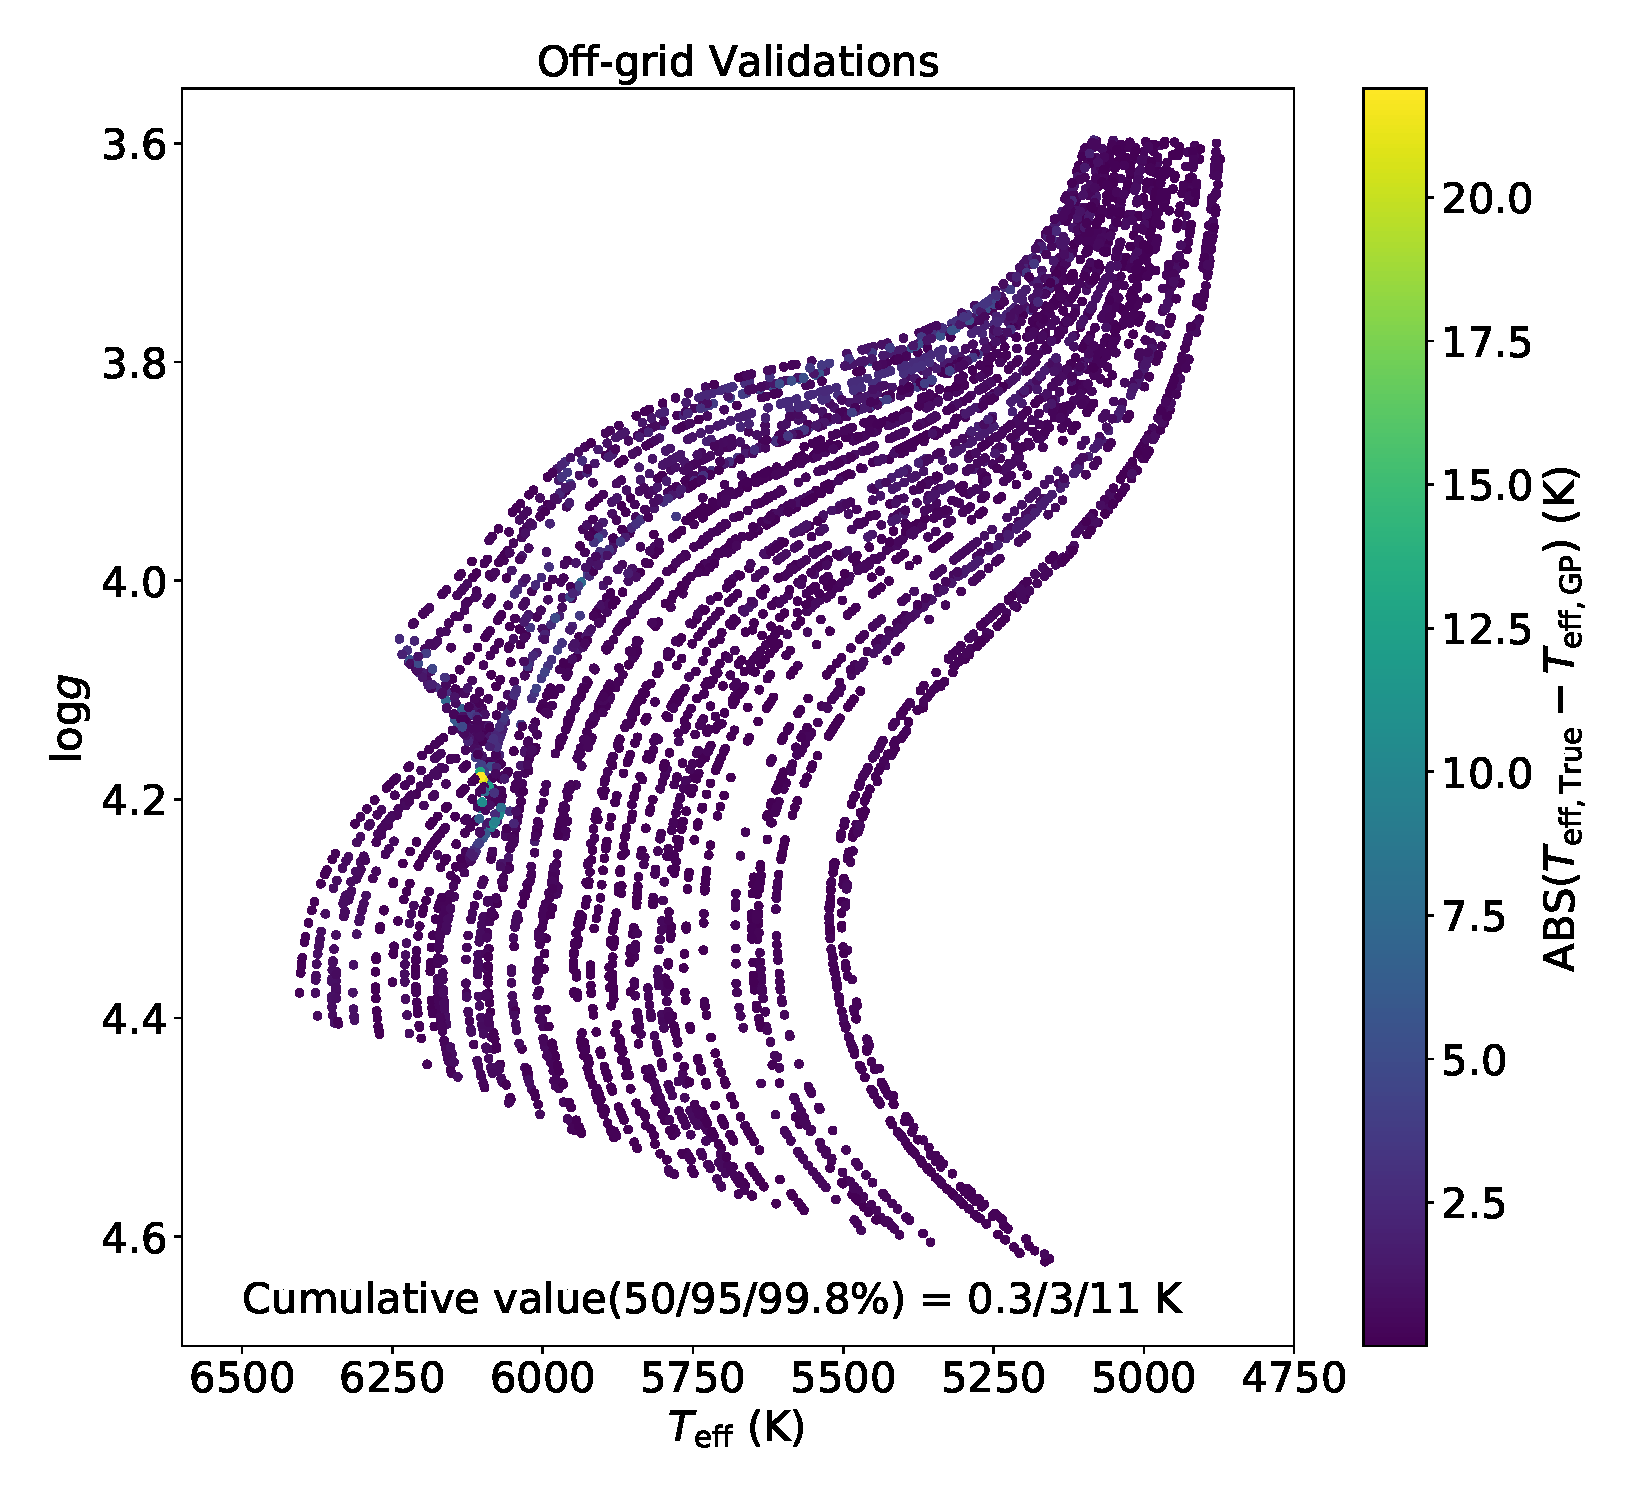
\includegraphics[width=1.0\columnwidth]{off_validation_hr.pdf}
    \caption{Off-grid validations.}  
    \label{fig:off-grid_validation}
\end{figure}


\subsubsection{Summary of the Work Flow}
 
\begin{figure}
	% To include a figure from a file named example.*
	% Allowable file formats are eps or ps if compiling using latex
	% or pdf, png, jpg if compiling using pdflatex
	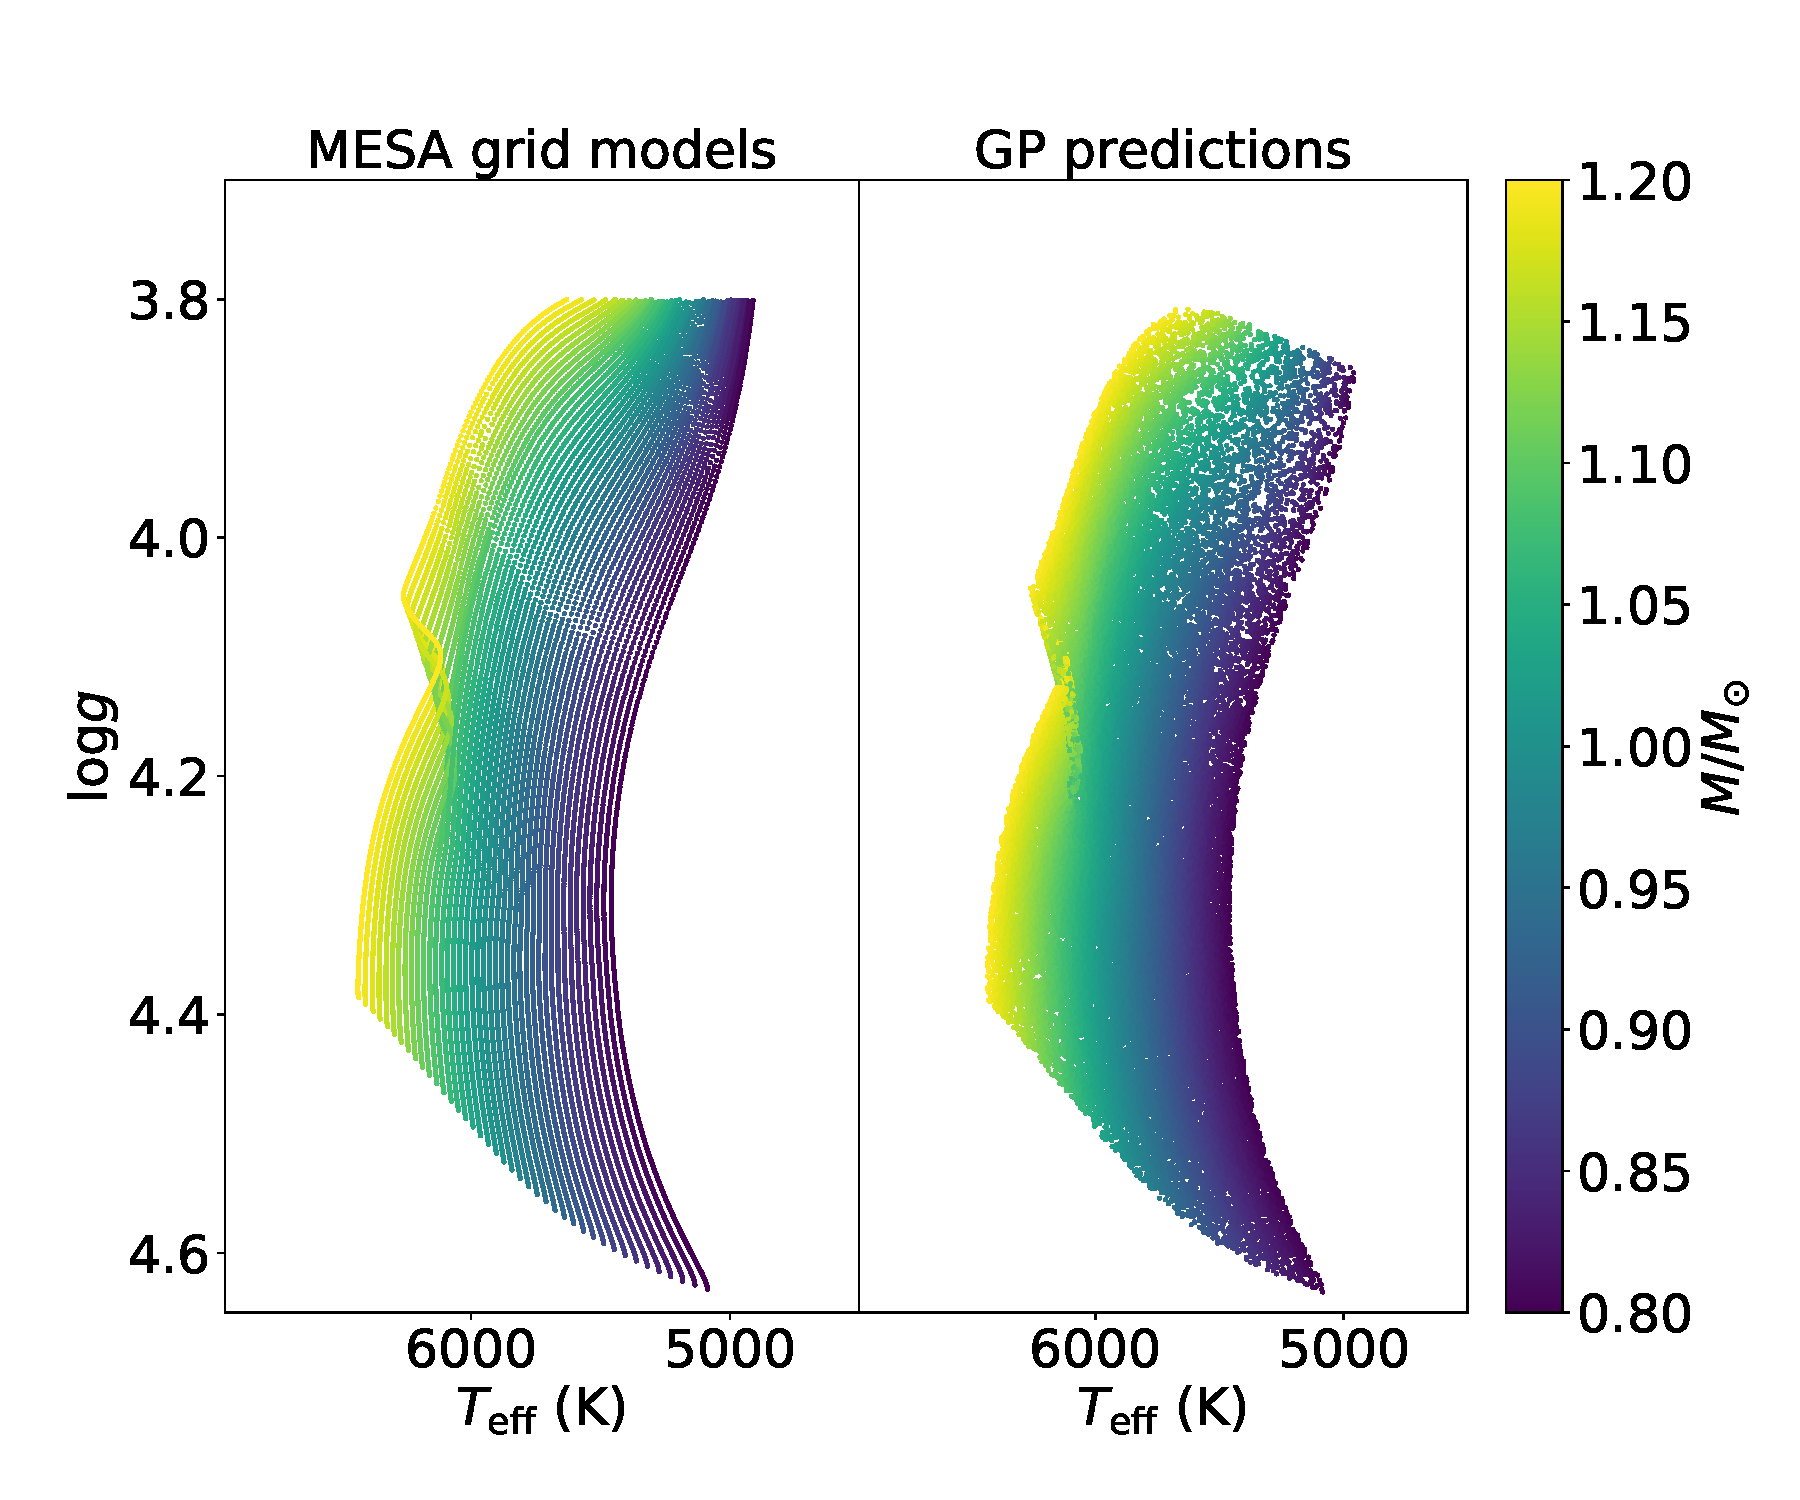
\includegraphics[width=1.0\columnwidth]{2d_hrd_compare.pdf}
    \caption{MESA grid models (sparse) and GP predictions (non-sparse) on the $T_{\rm eff}$ - $\log g$ diagram.}
    \label{fig:gpmodel}
\end{figure}


\subsection{The GPR model with Five-demission Inputs}

\begin{itemize}
\item Accuracy goes down. Because the multiple-demission space size increase while the training dataset has a limitation of 10,000 points.  
\item We hence need to divide the grid into small chunks and train each chunk separately.  (illustrate how chunks are divided)
\item  show training and validation results in a fancy way. 
\end{itemize}


\begin{table*}
	\centering
	\caption{Training and validating for the 5D GPR models}
	\label{tab:gpdetails}
	\begin{tabular}{lcc|cccccccc} % four columns, alignment for each
		\hline
		 GPR model inputs &\multicolumn{2}{c}{Training information} & \multicolumn{6}{c}{Validations of GPR outputs (50/95/99.8)}\\ % ($\sigma_{\rm val}$)}\\
		 \hline
		& $N_{\rm grid}$&$N_{\rm training}$&$\delta t$&$\delta \Delta\nu$& $\delta T_{\rm eff}$ & $\delta \log g$ & $\delta R$ & $\delta$[Fe/H]\\
		  & ($10^3$)& ($10^3$)& (Myr)&($\mu$Hz)&(K)&($10^{-3}$dex)&($10^{-3}R_{\odot}$)&($10^{-3}$dex)\\
		 \hline
		$M$, $t_{\rm frac}$, [Fe/H]$_{\rm init}$, $Y_{\rm init}$, $\alpha_{\rm MLT}$& 8,212 & 10 & 6/47/102& 0.06/0.4/1& 3/15/62&0.6/3/12&1/6/26&\\
       \hline
	\end{tabular}
\end{table*}







